\section{Методы управления параметрами.}

\begin{itemize}
    \item Правило "одной пятой" (один из вариантов)
    \begin{itemize}
        \item Рассматриваем (1 + 1)-ЭА
        \item Два гиперпараметра: $F > 1$ и $s$, управляем вероятностью мутации $p$
        \item Правило в общем виде:
        \begin{itemize}
            \item Потомок не хуже родителя: $p \leftarrow p · F$ 
            \item Потомок хуже родителя: $p \leftarrow p/F^{1/s}$
        \end{itemize}
        \item «Правило одной пятой»: $s= 4, F \approx 1.5$
        \begin{itemize}
            \item Стремится к тому, чтобы на одно улучшение приходилось $s$ итераций без улучшения. Тогда улучшение будет один раз в $s + 1$ итераций
        \end{itemize}
        \item «Правило 1/e»: $s= e-1, F = 1 + \frac{(logn)^2}{n}$ (\textbf{для F нужно уже другое значение})
    \end{itemize}
    \item 2-rate
    \begin{itemize}
        \item Для алгоритмов с дочерними популяциями, например, $(1 + \lambda)-ЭА$
        \item Поддерживаем вероятность мутации $p$ в пределах от $p_{min}$ до $1/2$
        \item На каждой итерации:
        \begin{itemize}
            \item Половину потомков создаем с вероятностью мутации $2p$
            \item Половину потомков создаем с вероятностью мутации $p/2$
            \item Пусть $p′$ — вероятность мутации, с которой был сгенерирован лучший потомок
            \begin{itemize}
                \item С вероятностью $1/2$ устанавливаем $p \leftarrow p′$
                \item Иначе меняем случайным образом или на $2p$, или на $p/2$
            \end{itemize}
        \end{itemize}
        \item Применяем ограничение: $p \leftarrow min(1/2, max(p_{min}, p ))$
        \item Тоже неплохо работает! Особенно для больших $\lambda$    
    \end{itemize}
\end{itemize}


\begin{figure}[h]
    \centering
    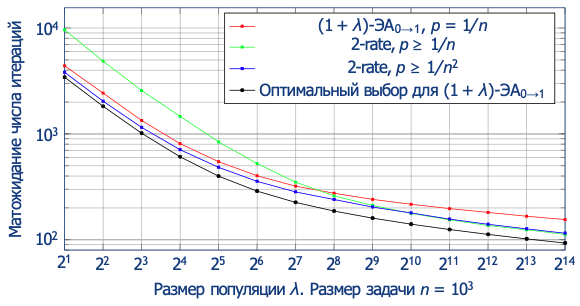
\includegraphics[width=0.8\linewidth]{images/c33_2rate.png}
    \caption{Пример}
    \label{fig:mpr}
\end{figure}
    